 \documentclass{article} %A4
\usepackage[a4paper,left=1.9cm, right=2.1cm,top = 1.2cm,bottom=2.3cm]{geometry}
\usepackage[utf8]{inputenc}%Umlaute
\usepackage[ngerman]{babel} %Texttrennung
\usepackage{graphicx}	%Grafiken
\usepackage{amssymb}
\usepackage{amsmath}
\usepackage{url}
\usepackage{listings}
\usepackage{color}
\usepackage{hyperref}
\usepackage{framed}
\usepackage{algpseudocode}
\usepackage{tikz}
\usepackage{enumitem}
\usepackage[xindy]{glossaries}
\makeglossaries
\usepackage[labelformat=empty]{caption}
\title{Zusammenfassung - Kryptographie}
\author{
	Marc Meier
}




\begin{document}
\maketitle
\begin{framed}Korrektheit und Vollständigkeit der Informationen sind nicht gewährleistet.
Macht euch eigene Notizen oder ergänzt/korrigiert meine Ausführungen!
\end{framed}
\setcounter{tocdepth}{1}
\tableofcontents

\section{Grundlagen}

% 010, 020
\subsection{Grundprinzipien und Entwicklung des Internets}
Das Internet entwickelte sich ab den 1960er Jahren.
Es ging aus dem am Ende des Jahrzehnts entstandenen, vornehmlich militärisch und akademisch geprägten ARPA-Net hervor.
Heutzutage wird es international kommerziell, industriell und auch akademisch (Katzenbilder) genutzt.
Bei seiner Entstehung war vor allem eine dezentrale Struktur ohne zentrale Verwaltung von Interesse.
Grund hierfür war die Angst des amerikanischen Department of Defense, dass eine atomarer Angriff zentrale Kommunikationspunkte außer Kraft setzen könnte.
Die Kommunikation findet über hochgradig vernetzte Knoten mithilfe von Paketen statt.

Literatur: \cite{abbate2000inventing, baran1964distributed}
\subsection{Packet Switching}
Paketvermittelte Übertragung bedeutet die Abkehr von der leitungsbasierten Vermittlung.
Dabei werden längere Nachrichten in Datenpakete aufgeteilt und voneinander unabhängig versendet.
Dies ermöglicht eine faire Verteilung der Leistungskapazität und redundante Wege bei einem Ausfall von Knoten oder Verbindungen.
Im Gegenzug können konstante Bandbreiten nicht ohne Weiteres (Abschnitt \ref{sec:qos}) gewährleistet werden, ebenso ergeben sich unterschiedliche Laufzeiten von Paketen.

\subsection{Dezentrale Verwaltung des Internets}

\subsubsection{Prinzipien}

\begin{itemize}
\item Keine zentrale Verwaltung oder Behörde (trotz Einflussnahme)
\item Demokratisches Zusammenwirken der Beteiligten / Wahlen
\item Selbstorganisation
\item Standards dort, wo sie erforderlich sind
\item Dynamisch, offen für Neuigkeiten	
\end{itemize}

\subsubsection{Organisationen}

\begin{description}
\item [ICANN:] Vergibt IP-Adressen und betreibt die DNS-Rootserver.
\item[IETF:] Standardisierung von Protokollen in RFCs \cite{rfc3233}
\item[RIPE:] Administration und technische Koordination
\item[RIPE NCC:] Adressvergabe in Europa und Zentralasien, Verwaltung der WHOIS-Datenbank.
\item[DENIC eG:] Domain-Verwaltung für die Zone .de
\end{description}

\subsection{Standards}
Standards ermöglichen die Kooperation im Netzwerk, nur durch sie können Geräte verschiedener Hersteller miteinander kommunizieren.
Sie können textuell, mithilfe einer Referenzimplementierung oder anhand von Automaten (meist für zustandsbehaftete Protokolle) festgelegt werden.

\begin{description}
\item[Protokoll] Standardisierte Regeln (Vorschriften) und Vereinbarungen zu
Form, Ablauf, Steuerung und Sicherung (Fehler) der
Datenübertragung in und zwischen Rechnernetzen, zwischen
Einzel-Rechnern und zwischen Rechnern und
Peripheriegeräten.
\item[Standard] Ein Standard wird von den verschiedensten internationalen und
nationalen Organisationen sowie von großen Firmen erstellt.
Ein Standard wird als verbindliche oder unverbindliche
(empfohlene) Festlegungen schriftlich niedergelegt.
\end{description}

Ablauf einer Standardisierung bei RFCs:
\begin{enumerate}
	\item \textbf{Proposed Standard}: Vollständige, konsistente Spezifikation vorhanden
	\item \textbf{Draft Standard}: Mindestens 2 unabhängige, interoperable Implementierungen
	\item \textbf{Standard}: Operationell stabil
\end{enumerate}
\textbf{Weitere Status:} \emph{Experimental}, \emph{Informational} und \emph{Historic}.
\subsection{Netze, Autonome Systeme und Schichten}
Große Teile des Internet-Backbones werden von wenigen Firmen bereitgestellt (Tier-1).
Diese werden an einigen Knotenpunkten verbunden.
Wichtiger Knotenpunkt in Deutschland ist DE-CIX in Frankfurt/Main.
Man unterteilt folgende \textbf{Netzwerk-Schichten}:
\begin{description}
	\item[Tier 1]: Ein Netzwerk, das mit allen anderen Tier-1-Netzwerken verbunden ist; \emph{Internet-Backbone}; z.B. ATDN, GX, AT\&T...
	\item[Tier 2]: Netzwerk, das mit vielen Netzwerken verbunden ist, aber Transit \emph{einkauft}, um einige Bereiche des Internets zu erreichen; z.B. Deutsche Telekom
	\item[Tier 3]: Ein Netzwerk, das ausschließlich Transit \emph{einkauft}, um das
	Internet zu erreichen
\end{description}
\textbf{Autonome Systeme} sind Ansammlungen von IP-Netzen, die als Einheit verwaltet werden.
Innerhalb kommt ein einheitliches Routing-Protokoll zum Einsatz.
Autonome Systeme sind untereinander verbunden und
bilden das Internet.
\section{Protokolle}

\subsection{Zustandslose und zustandsbehaftete Protokolle}
Bei \textbf{zustandslosen Protokollen} wird jede Anfrage in einer eigenständigen Transaktion ausgeführt, es existieren keine Vorbedingungen oder Sitzungsinformationen (UDP, HTTP, TFTP).
\textbf{Zustandsbehaftete Protokolle} hingegen merken sich den aktuellen Zustand mithilfe einer Sitzung.
Nachfolgende Anfragen können auf die Sitzungsinformationen zugreifen.
Diese Zustandsübergänge können durch endliche Automaten dargestellt werden.
Beispiele sind FTP, TCP und SMTP.

\subsection{OSI-7-Schichten-Modell}

\begin{enumerate}
	\item Physical Layer / Bitübertragung
	\item Data Link Layer / Sicherungsschicht / Datenübertragungsschicht
	\item Network Layer / Vermittlungsschicht
	\item Transport Layer
	\item Session Layer / Sitzungsschicht
	\item Presentation Layer / Darstellungsschicht
	\item Application Layer / Anwendungsschicht
\end{enumerate}

Gute \textbf{Eselsbrücken} sind:
\begin{itemize}
	\item Alle deutschen Studenten trinken verschiedene Sorten Bier (deutsche Bezeichnungen, 7-1)
	\item An dem Samstag trug Verena 'nen String in Blau (deutsche Bezeichnungen, 7-1)
	\item Alle poppen Susis Tante nach der Party (deutsche Bezeichnungen, 7-1)
	\item Physiker, die nicht trinken sind potentielle Attentäter (deutsche/englische Bezeichnungen, 1-7)
	\item Alibaba präsentiert sich täglich nackt dem Personal
	\item  Please Do Not Throw Salami Pizza Away (englisch, 1-7)
\end{itemize}

Jede Schicht $n$ nutzt die darunterliegende Schicht $n-1$ um mit dem Kommunikationspartner zu kommunizieren.
Daten höherer Schichten werden in niederen Schichten umkapselt.
Die Bezeichnung der Pakete ist je nach Schicht unterschiedlich:
\begin{description}
	\item[Data Link Layer]: (Ethernet-)Frame
	\item[Network Layer]: Paket
	\item[Transport Layer]: Fragment
\end{description}

\subsection{Ethernet}

Das Ethernet-Protokoll wirkt auf den Layern 1 + 2 und wird im Standard \textbf{IEEE 802.3} definiert.
Es kümmert sich um Elektrokrams (Physikalische Eigenschaften, Stecker,Stromversorung, Kabel etc.), Zugriffsverfahren auf das Medium, Adressierung (MAC), Protocol-Multiplexing, Flow Control (Logical Link Control) und Fehlererkennung (CRC).
Es ähnelt den Standards \textbf{802.11} (WLAN), \textbf{802.15.1} (Bluetooth) und \textbf{802.16} (WiMAX).

Ein \textbf{Ethernet-Frame} hat eine Größe von 64 - 1518 Byte.
Davon ausgenommen sind die Präambel und der SFD.
Wird das VLAN-Tag genutzt, sind 1522 Byte möglich.
Das \textbf{Ethernet-Paket} (Offensichtlich Präambel + SFD + Ethernet-Frame) umfasst folgende Felder:

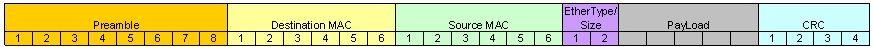
\includegraphics[width=16cm]{img/EthernetFrame.jpg}

\begin{description}
	\item[Präambel]: Zum Synchronisieren von Sender und Empfänger, \emph{Einschwingphase} (8 Byte)
	\item[SFD]: Festgelegte Sequenz 10101011 (1 Byte)
	\item[Ziel-Mac-Adresse]: Adresse des Empfängers (8 Byte)
	\item[Quell-Mac-Adresse]: Adresse des Senders (8 Byte)
	\item[VLAN-Tag]: Nach IEEE 802.1q, optional (4 Byte)
	\item[Typ-Feld]: Identifiziert die Art des nachfolgenden Inhalts, z.B. IP, ARP, etc...
	\item[Nutzlast]
	\item[PAD-Füllfeld]: Wird optional benötigt, um die Mindestlänge von 64 Byte einzuhalten \footnote{Rausfinden, warum mindestens 64 Byte nötig. Vermutung: Kollisionserkennung}
	\item[CRC-Prüfsumme]: Zur Fehlererkennung (4 Byte)
\end{description}

\subsubsection{CSMA/CD}

CSMA/CD regelt den Zugriff auf ein von mehreren Teilnehmern genutztes Medium (Kabel).
Dazu prüft der sendene Host, ob das Medium frei ist, bevor er sendet.
Beim Übertragen von Daten können Kollisionen erkannt werden.
Der Sendevorgang wird dann nach einer zufälligen Zeit wiederholt.
Aufgrund der verbreiteten Nutzung von Switches sind echte geteilte Medien inzwischen eher die Ausnahme.

$\Rightarrow$ Jeder Port am Switch bildet eine eigene \emph{Kollisionsdomäne}.
Die Bustopologie mit Koaxialkabeln (aber auch mit Hubs) wird nicht mehr genutzt.

\subsubsection{Duplex / Half Duplex}

Beim \textbf{Full Duplex} sind beide Seiten in der Lage, gleichzeitig zu Senden und zu Empfangen.
Im Falle von \textbf{Half Duplex} ist dies nur wechselseitig möglich (vgl Walkie Talkie).
Es sind verschiedene Realisierungen einer geteilten Nutzung eines Mediums möglich:

\begin{description}
	\item [Zeitduplex (TDD)]: Übertragung in verschiedenen Zeitschlitzen
	\item [Frequenzduplex (FDD)]: Übertragung auf verschiedenen Frequenzen
	\item [Codeduplex]: (nicht im Skript)
\end{description}

\subsection{Switching}

\textbf{Switches} sind Geräte auf dem OSI-Layer 2.
Sie empfangen Ethernet-Frames und leiten sie anhand ihrer Empfänger-MAC-Adresse weiter.
Im Gegensatz zum Hub wird dabei nur über den Port ausgegeben, hinter dem sich der Empfänger befindet.
Die Ausnahme ist hierbei, wenn der Port des Empfängers nicht bekannt ist.
Anhand der empfangenen Frames lernt ein Switch, wo sich Geräte befinden.

\subsubsection{Realisierungsmöglichkeiten}

%TODO

\subsubsection{Cut-Through und Store-and-Forward}

Beim \textbf{Cut-Through} (auch \emph{On The Fly Forwarding}) werden Pakete sofort nach Empfang der Empfängeradresse auf dem entsprechenden Port weitergeleitet, sofern dieser Frei ist.
Diese Methode ist sehr schnell (Verzögerung ca. 40$\mu$s), leitet jedoch gegebenenfalls auch fehlerhafte Frames weiter, da CRC umgangen wird.

\textbf{Store-and-Forward} hingegen empfängt zuerst den gesamten Frame, prüft diesen und leitet ihn anschließend weiter.
Offensichtlich werden keine fehlerhaften Pakete mehr in benachbarte Segmente weitergeleitet, dies wird jedoch durch erhöhte Latenz erkauft.

In der Praxis arbeiten Switches häufig im Cut-Through-Modus und schalten bei erhöhter Fehlerrate in den Store-and-Forward-Modus.

\subsubsection{VLAN}

Ermöglicht die Aufteilung von Switches in mehrere virtuelle LANs.
Den Ports werden dabei einzelne VLANs zugeordnet.
Auf diese Weise kann Hardware eingespart werden.
Realisiert wird dies mit einem 4 Byte langen Feld im Ethernet-Frame:
\begin{itemize}
	\item 2 Bytes \textbf{TPID} - Tag Protocol Identifier – Fester Wert 0x8100. Frame
	trägt die 802.1Q/802.1p-Tag-Information
	\item 3 Bit \textbf{Priorität} (user\_priority) – Benutzer-Prioritätsinformationen
	\item 1 Bit \textbf{CFI} - Canonical Format Indicator – Gilt für alle vorhandenen
MAC-Adressinformationen im MAC-Datenpaket des Frames. Wert 0
das Format ist kanonisch (am wenigsten signifikante Bit zuerst); Wert
1 Format nicht-kanonisch. Benutzung im Token Ring/Source-Routed-
FDDI-Media-Zugang, um die Bit-Order der Adressinformationen des
verkapselten Frames festzulegen
	\item 12 Bit \textbf{VID} - VLAN Identifier – Identifizierung des VLANs zu dem der
Frame gehört
\end{itemize}

\subsubsection{Trunking / Link Aggregation}
Ermöglicht die Zusammenfassung mehrerer Ports zur Erhöhung des Datensatzes.

\subsection{Asynchronous Transfer Mode}

\subsection{Internet Protocol}

\subsubsection{IPv4}

\subsubsection{IPv6}

\subsection{User Datagram Protocol}

\subsection{Transmission Control Protocol}

\section{Adressierung}

% 030

\section{ARP, RARP}

% 040

\section{DNS und WHOIS}

% 050

\section{Migration von IPv4 nach IPv6}

% 060

\section{Timeouts, ACK, Bestätigungen}

% 070

\section{Routingkonzepte}

% 080, 090, 095, 100, 110, 120, 130

\section{Quality of Service}
\label{sec:qos}
% 140

\section{Multicasts}

% 150, 180

\section{Zeitsynchronisation}

% 160, 190

\section{Internet Control Message Protocol}

% 170

\section{Voice over IP}

% 200, 210

\section{World Wide Web und HTTP}

% 220, 230

\section{Peer-to-Peer}

% 240, 250

\section{E-Mail}

% 260

\section{Autokonfiguration}

% 280, 290

\section{Dateien und Drucken}

% 300, 310

\section{Telnet, SSH und rlogin}

% 320

\section{Extensible Messaging and Presence Protocol (XMPP)}

% 330

\section{LDAP}

% 340

\section{Authentication Protocols}

% 350

\section{Simple Network Management Protocol}

% 360 

\section{Mac-Sublayer}

% 365

\section{Mobile Netzwerke}

% 370, 380, 390, 400

\section{HTTP2 und SCTP}

% 410


\newpage
\addcontentsline{toc}{section}{Literatur}
\bibliographystyle{plain}
\bibliography{literatur}


\newglossaryentry{arpa}{name=ARPA,description={Advanced Research Projects Agency}}
\newglossaryentry{icann}{name=ICANN,description={Internet Corporation for Assigned Names and Numbers}}
\newglossaryentry{ietf}{name=IETF,description={Internet Engineering Task Force}}
\newglossaryentry{ripe}{name=RIPE,description={Réseaux IP Européens}}
\newglossaryentry{ripencc}{name=RIPE NCC,description={Réseaux IP Européens Network Coordination Centre}}
\newglossaryentry{denic}{name=DENIC,description={Deutsches Network Information Center}}
\newglossaryentry{dns}{name=DNS,description={Domain Name System}}
\newglossaryentry{udp}{name=UDP,description={User Datagram Protocol}}
\newglossaryentry{tcp}{name=TCP,description={Transmission Control Protocol}}
\newglossaryentry{atdn}{name=ATDN,description={AOL Transit Data Network}}
\newglossaryentry{gx}{name=GX,description={Global Crossing}}
\newglossaryentry{decix}{name=DE-CIX,description={German Commercial Internet Exchange}}
\newglossaryentry{http}{name=HTTP,description={Hypertext Transfer Protocol}}
\newglossaryentry{tftp}{name=TFTP,description={Trivial File Transfer Protocol}}
\newglossaryentry{ftp}{name=FTP,description={File Transfer Protocol}}
\newglossaryentry{smtp}{name=SMTP,description={Simple Mail Transfer Protocol}}
\newglossaryentry{mac}{name=MAC,description={Medium Access Control}}
\newglossaryentry{crc}{name=CRC,description={Cyclic Redundancy Check}}
\newglossaryentry{csmacd}{name=CSMA/CD,description={Carrier Sense Multiple Acces / Collision Detection}}
\newglossaryentry{fdd}{name=FDD,description={Frequency Divsion Duplex}}
\newglossaryentry{tdd}{name=TDD,description={Time Division Duplex}}
\newglossaryentry{sfd}{name=SFD,description={Start Frame Delimiter}}
\newglossaryentry{atm}{name=ATM,description={Asynchronous Transfer Mode}}
\newglossaryentry{tpid}{name=TPID,description={Tag Protocol Identifier}}
\newglossaryentry{cfi}{name=CFI,description={Canonical Formati Indicator}}
\newglossaryentry{vid}{name=VID,description={VLAN Identifier}}
\newpage
\addcontentsline{toc}{section}{Glossar}

\printglossary[title=List of Terms,toctitle=Terms and abbreviations]

\end{document}